\vspace{5cm}
\section{Arquitectura Cliente-Servidor}
Desde el punto de vista funcional, se puede definir la computación Cliente/Servidor como una arquitectura distribuida que permite a los usuarios finales obtener acceso a la información en forma transparente aún en entornos multiplataforma \cite{clientServ}
\\\newline
\begin{figure}[H]
\centering
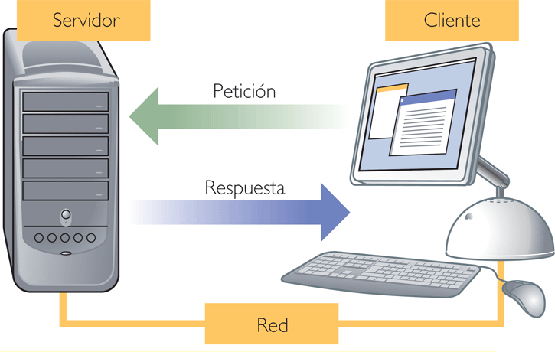
\includegraphics[width=0.4\textwidth]{imagenes/servidor1}
\caption{Arquitectura Cliente-Servidor}
\label{img:clientserv}
\end{figure}
    
\subsection{Cliente}
El Cliente normalmente maneja todas las funciones relacionadas con la manipulación y despliegue de datos, por lo que están desarrollados sobre plataformas que permiten construir interfaces gráficas de usuario (GUI), además de acceder a los servicios distribuidos en cualquier parte de una red. \cite{clientServ} 
\\\newline
\subsection{Servidor}
Es el proceso encargado de atender a múltiples clientes que hacen peticiones de algún recurso administrado por él. Al proceso servidor se le conoce con el término back-end.
El servidor normalmente maneja todas las funciones relacionadas con la mayoría de las reglas del negocio y los recursos de datos. \cite{clientServ}
\vfill